\documentclass[a4paper]{extarticle}
\usepackage[utf8]{inputenc}
\usepackage{hyperref}
\usepackage{geometry}
\usepackage{fancyhdr}
\usepackage{graphicx} % libreria per le immagini
\usepackage{amssymb} %libreria per i simboli (ex. alfabeto reco)
\usepackage{algorithm2e} %libreria per scrivere pseudocodice
\usepackage{longtable}
\usepackage{caption}
\usepackage{lastpage}

\setlength{\parindent}{0em}%indentazione paragrafo
\setlength{\parskip}{1em}%spazio tra paragrafi
\renewcommand{\baselinestretch}{1.3}%interlinea
\graphicspath{ {./} }
\geometry{
    a4paper,
    left=10mm,
    right=10mm,
    bottom=20mm
}


\hypersetup{
    colorlinks=true,
    linkcolor=blue,
    filecolor=blue,      
    urlcolor=blue,
    pdftitle={Overleaf Example},
    pdfpagemode=FullScreen
}

\pagestyle{fancy}
\fancyhf{}
\rhead{Federico Calò}
\lhead{Data Mining - Il processo KDD}
\cfoot{  \thepage }


\title{Data Mining - Il processo KDD}
\author{\href{http://www.federicocalo.it}{Federico Calò} }
\date{}

\begin{document}
\maketitle
\newpage
\tableofcontents
\voffset -30pt

\newpage

\section{KDD process}

L'automazione delle attività economiche produce un incremento dello stream di dati perchè anche singole transazioni (una chiamata telefonica, il credito di una carta, un test medico) sono tipicamente registrate in un computer.
Le basi di dati scientifiche e governative sono anche in rapida crescita. C'è un divario crescente tra la generazione di dati e la loro comprensione. Risulta quindi necessario l'utilizzo di computer per analizzare i dati, ma questo non è sufficiente.

Necessitiamo di una metodologia matura che spieghi come grandi strutture di dati possono essere analizzate. Questa metodologia è stata studiata in un'area di ricerca conosciuta come KDD. Lo scopo è investigare come tecniche di Machine Learning possono 
essere applicate a estratti di "conoscenza" di una grande massa di dati disponibili. All'inizio vi era una certa confusione sull'area di interesse ricoperta dal Machine learning, Data Mining e Knowledge Discovery. 
Ora, si è giunti alla conclusione che il KDD denota l'intero processo di estrazione della conoscenza, dalla raccolta dei dati e dalla preelaborazione all'interpretazione dei risultati.

Il Data Mining è lo step, all'interno del processo KDD, nel quale le informazioni sono estratte dai dati applicando ad essi opportuni algoritmi. Questi algoritmi sono il più delle volte quelli di Machine Learning. 
In un contesto aziendale il termine Data Mining è ancora utilizzato per denotare il processo di knowledge discoverym e questo causa qualche confusione. Sempre sulla terminologia: KDD è ancora utilizzato anche se la conoscenza non è rigorosamente estratta dai "database". 

Il tentativo più importante e completo di definire il Knowledge Discovery come un processo afferma: "La scoperta della conoscenza è l'estrazione non banale di informazioni implicite, precedentemente sconosciute e potenzialmente utili dai dati."
\begin{itemize}
    \item \textbf{Non banale}: si intende che nel processo è coinvolta qualche ricerca o inferenza statistica, quindi non è un semplice calcolo di quantità predefinite;
    \item \textbf{Implicita}: ci si riferisce al fatto che l'informazione è implicita nel dato e non formalmente esplicita, l'informazione esplicita è estratta attraverso altre tecniche;
    \item \textbf{Sconosciuta}: l'informazione deve essere nuova, la novità dipende dal quadro di riferimento assunto;
    \item \textbf{Utile}: l'informazione deve essere utile a raggiungere lo scopo del sistema o dell'utente. I pattern completamente estranei agli obiettivi dati sono di scarsa utilità e non costituiscono conoscenza all'interno della situazione data.
\end{itemize}

Diamo una definizione formale al KDD:

\textbf{Dati}:
\begin{itemize}
	\item un insieme di fatti (data) F,
	\item una rappresentazione in un linguaggio L,
	\item una certa misura di certezza C,
\end{itemize}
possiamo definire un pattern come una dichiarazione S in L che descrive le relazioni tra un sotto insieme $F_{S}$ di F con una certezza \textbf{\textit{c}}, tale che S è più semplice (in un certo senso) dell'enumerazione di tutti i fatti in $F_S$.

Un pattern è considerato conoscenza se è interessante e abbastanza
certo (o valido). Nel KDD siamo interessati in pattern che sono espressi in un linguaggio di alto livello, come:
\newpage
\begin{center}
Se Età $<$ 25 e Corso-di-Educazione = no

Allora Incidente = si

Con probabilità = 0.2 a 0.3
\end{center}
In questo modo alcuni pattern possono essere capiti e usati direttamente dalle persone o possono essere input ad altri programmatori.
Definiamo ora il termine \textbf{certezza}, senza un livello sufficiente di certezza i modelli diventano ingiustificati e non riescono a diventare conoscenza. La certezza coinvolge diversi fattori, quali: 
\begin{itemize}
	\item Integrità dei dati,
	\item Dimensione del campione su cui è stata effettuata la scoperta 
	\item Il grado di supporto dalla conoscenza del dominio disponibile
\end{itemize}

Un pattern è definito \textbf{interessante} quando è:
\begin{itemize}
	\item Nuovo
	\item Utile
	\item Non banale da calcolare
\end{itemize}

Vi sono principalmente due differenti interpretazioni dei pattern e dei modelli.
La \textbf{prima} interpretazione che possiamo dare consiste nel definire un modello come una sintesi globale del data-set, mentre il pattern è una caratteristica locale del data-set, limitato a un sub-set di osservazioni e/o attributi.
La \textbf{seconda interpretazione} esplica come il data mining implica l'adattamento o la determinazione di pattern da dati osservati. In questo caso il pattern è visto come una istanza del modello. I modelli adattati svolgono il ruolo di conoscenza dedotta

Il kdd è un processo iterativo e interattivo, costituito da molti passaggi che includono molte decisione prese dall'utente.

\begin{figure}[h]
\noindent
\makebox[\textwidth]{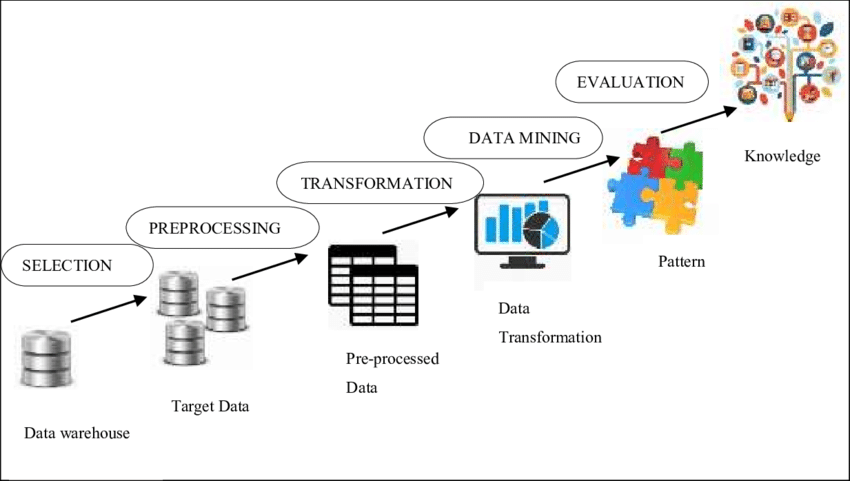
\includegraphics[width=12cm]{kdd-process}}%
\end{figure}

In una prima fase si sviluppa una \textbf{comprensione del dominio} dell'applicazione, delle relative conoscenze di base e degli obiettivi dell'utente finale. Si prosegue creando \textbf{un data set target}, quindi si seleziona un dataset o ci si focalizza su un sotto insieme di variabili o di esempi di dati sui quali deve essere eseguita la scoperta. Una volta selezionati questi dati si passa alla fase di \textbf{pulizia dei dati e preprocessing} nella quale si effettuano svariate operazioni volte a rimuovere il rumore o dei valori anomali, collezionando le informazioni necessarie per modellare o tenere conto del rumore, decidere strategie per gestire i campi di dati mancanti o tenere conto delle informazioni sulla sequenza temporale e delle modifiche note. Successivamente si entra in una fase di \textbf{riduzione e proiezione dei dati}, nella quale si trovano funzioni utili per rappresentare i dati a seconda dell'obiettivo dell'attività. Vengono utilizzati metodi di riduzione o trasformazione multidimensionale per ridurre l'effettivo numero di variabili da considerare o per trovare rappresentazioni di dati invarianti. Conclusa questa attività, si passa alla \textbf{selezione del compito del data mining}, decidendo qual è l'obiettivo del processo KDD, scegliendo tra classificazione, regressione, clustering. 

Definito l'obiettivo si passa alla \textbf{scelta degli algoritmi} di data mining. Vengono selezionati i metodi che verranno utilizzati per ricercare i pattern frequenti all'interno dei dati. Vengono definiti i modelli e i parametri più appropriati e si cerca di far corrispondere particolari metodi di data mining con i criteri globali dei processi di KDD. Quindi si entra nella fase di \textbf{Data Mining}, nella quale si ricercano modelli di interesse in una particolare forma rappresentativa.  L'utente può contribuire significativamente in questa fase eseguendo correttamente i passaggi precedenti. Alla fine del processo di data mining, vi è la fase di \textbf{interpretazione dei pattern minati}, nella quale si effettuano le valutazioni sui risultati ottenuti ed eventualmente si ritorna ad iterare su uno degli step precedenti. Infine si \textbf{consolida la conoscenza scoperta}, la conoscenza ottenuta viene incorporata nel sistema per migliorarne le prestazioni o semplicemente si documenta per essere segnalata ad altre parti di interesse. Questa fase include anche il controllo e la risoluzione di particolar conflitti con conoscenze precedentemente estratte o scoperte.

\subsection{Steps del KDD}

La maggior parte del lavoro nel KDD è focalizzata sullo step del data mining. Anche se gli altri step sono considerati importanti per il successo dell'applicazione del KDD nella pratica. La necessità per una standardizzazione del processo della scoperta della conoscenza ha portato alla definizione dello standard industriale CRISP-DM. L'obiettivo di questo standard è quello di sviluppare un processo neutrale per condurre il KD,  e di definire i compiti, i loro outputs, la terminologia e i problemi tipici di caratterizzazione. 

Il modello di processo CRISP-DM è per la scoperta i conoscenza consiste in sei fasi.

\fbox{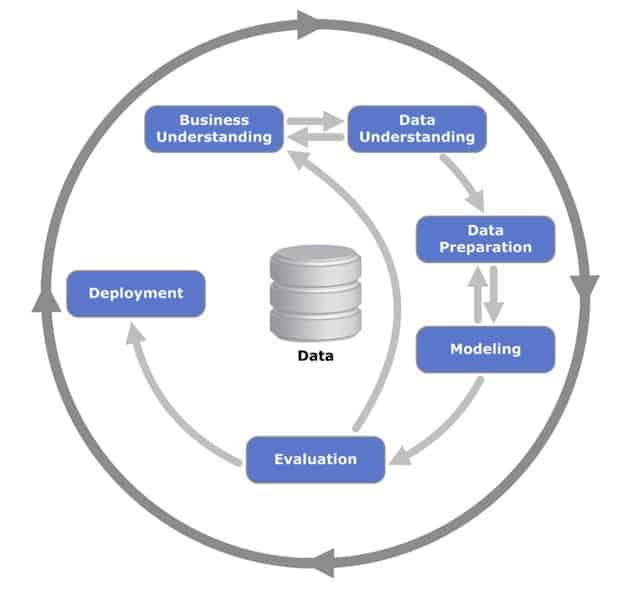
\includegraphics[width=.4\textwidth, height=.3\textheight, keepaspectratio]{crisp-dm-model}}




La sequenza delle fasi non è rigida. È possibile spostarsi avanti e indietro tra le diverse fasi a seconda dell'esito di ciascuna fase. Le frecce indicano le dipendenze più importanti/frequenti. Il cerchio esterno simboleggia la natura ciclica di un processo KDD che può continuare dopo l'implementazione di una soluzione. Ogni fase contiene un numero di task che produce specifici output.
\subsubsection{Business Understanding}
La \textbf{prima fase} di questo modello viene definita \textbf{Business Understanding} (comprensione degli affari), il cui primo step è quello di \textbf{determinare gli obiettivi commerciali}, step ha molti aspetti in comune con la fase iniziale di quasiasi impegno progettuale significativo. I requisiti minimi sono:
\begin{itemize}
	\item un problema o un'opportunità commerciale percepita
	\item un certo livello di sponsorizzazione esecutiva
\end{itemize}
Sviluppare una definizione chiara e comprensibile dei bisogni aziendali non è un compito semplice. E' richiesta la collaborazione dei business analyst e dei data analyst. Questo passaggio del processo è anche il momento in cui iniziare a definire le aspettative. Alla fine di questo step vengono prodotti:
\begin{itemize}
	\item \textbf{Il background}, che descrive le informazioni note sulla situazione aziendale all'inizio del processo
	\item \textbf{Gli obiettivi di business}, che descrivono i principali obiettivi dalle prospettive di business
	\item \textbf{I criteri economici di successo}, che definiscono le misure per risultati di alta qualità del progetto dal punto di vista del business
\end{itemize}

Dopo aver definito gli obiettivi commerciali, si passa alla \textbf{valutazione della situazione}, con lo scopo di raccogliere informazioni sulle risorse, sui vincoli e sulle assunzioni. Alla fine di questo sotto processo verrà prodotto un inventario contenente:
\begin{itemize}
\item le risorse: personale, dati, calcoli
\item vincoli: schede di compilazione, questioni legali, comprensibilità
\item assunzioni: disponibilità dei dati
\end{itemize}

Inoltre non dimentichiamo che vengono prodotti anche \textbf{un glossario di termini}, che copre la terminologia di business e di data mining, e \textbf{un'analisi costo-beneficio}, cioè un documento contenente le spese del progetto dovrebbero essere confrontate con i potenziali guadagni.

Successivamente si passa alla \textbf{determinazione degli obiettivi del Data Mining}. In questa fase si trasformano gli obiettivi commerciali in obietti del processo di Data Mining e si costruiscono i relativi criteri di successo. Possiamo classificare gli obiettivi del Data Mining in:
\begin{itemize}
\item Classification
\item Estimation (produrre una stima, Estimation)
\item Prediction
\item Affinity grouping
\item Clustering
\item Description e Profiling
\end{itemize}

I due obiettivi primari del Data Mining tendono ad essere:
\begin{itemize}
\item \textbf{Predizione}, che include l'uso di alcune variabili indipendenti per predire valori sconosciuti o futuri che dipendono da altre variabili
\item \textbf{Descrizione}, nella quale non si fa una distinzione tra variabili dipendenti e indipendenti e si concentra sulla ricerca di modelli interpretabili dall'uomo che descrivono i dati.
\end{itemize}
L'obiettivo della classificazione è apprendere una funzione che mappa, o classifica, un dato in una predefinita classe. Questa tecnica è molto utilizzata per i database. Invece quando si parla di regressione, si ha come obiettivo apprendere una funzione che mappa un dato in una variabile di previsione reale. Quando invece si cerca di creare un procedimento per trovare le associazioni tra gruppi di variabili, si utilizza il metodo Affinity Grouping. Il clustering è un'attività descrittiva in cui si cerca di identificare un insieme finito di categorie o cluster per descrivere i dati. Le categorie possono essere mutuamente esclusive ed esaustive, oppure consistere in una rappresentazione più ricca come una gerarchia o categorie sovrapposte. La clasterizzazione viene utilizzata spesso per scoprire sotto-popolazioni omogenee, identificare sotto categorie, o analisi di dati. Strettamente correlato al clustering è il compito della stima della densità di probabilità, che consiste in tecniche per stimare dai dati la funzione di densità di probabilità multivariata congiunta di tutte le variabili/campi nel database.
Per \textbf{Summarization} (riassunto o descrizione o profilazione), si intendono tutti quei metodi per trovare una descrizione compatta per un sottoinsieme di dati. Invece il task \textbf{Dependency modeling} (modellare le dipendenze), consiste nel trovare un modello che descrive dipendenze significative tra variabili. Esistono due tipi di modelli dipendenti:
\begin{itemize}
\item il livello strutturale di specifici modelli le cui variabili sono localmente dipendenti tra loro
\item il livello quantitativo il cui modello specifica quanto le variabili sono dipendenti usando una scala numerica.
\end{itemize}
Il task di rilevamento di modifiche e deviazioni si focalizza sulla scoperta delle modifiche più significanti nei dati rispetto a valori misurati o normativi in precedenza. Consiste nel trovare un modello che descrive significanti dipendenze tra variabili.

Dopo aver definito il task del Data Mining si passa a \textbf{produrre un piano progettuale} per il raggiungimento egli obiettivi di data mining e quindi il raggiungimento degli obiettivi di business. L'output di questa fase è ovviante un piano progettuale, che specifica l'insieme degli step per la restante parte del progetto, la sua durata, le risorse richieste, gli input, gli output e le dipendenze.

\subsubsection{Data Understanding}

Dopo aver contestualizzato il business in cui si andrà a progettare il sistema, si passa a una fase di \textbf{Data Understanding}, cioè di compresone dei dati, che inizia con una fase di raccolta iniziale dei dati, durante la si accede ai data rilevanti nell'inventario delle risorse e si produce un report iniziale dei dati raccolti, nel quale si elenca la posizione dei dati, i metodi usati per acquisirli e i problemi incontrati. Successivamente si passa a descrivere i dati esaminando le loro proprietà e creando un report nel quale si descrive il formato dei dati, i potenziali valori, la quantità, l'identificatore dei campi e tutte le caratteristiche che vengono scoperte.

Ci sono due metodi principali per descrivere le variabili:
\begin{itemize}
\item \textbf{in maniera categorica}: i possibili valori finiti e i differenti tipi che una variabile può assumere. Questa categoria si può suddividere in:
\begin{itemize}
\item \textbf{variabili nominali} che denominano il tipo di oggetto a cui si riferiscono, ma non esiste un ordine tra i valori possibili. (stato del materiale, genere, livello di educazione)
\item \textbf{variabili ordinali} che assumono un ordine tra i possibili valori. (valutazione del cliente)
\end{itemize}

\item \textbf{quantitativi}: sui quali sono consentite operazioni aritmetiche, e si suddividono a loro volta in:
\begin{itemize}
\item \textbf{variabili discrete}, i cui valori sono interi
\item \textbf{variabili continue}, i cui valori sono numeri reali.
\end{itemize}
\end{itemize}

Dopo aver descritto la tipologia di dati si passa alla verifica della loro qualità ispezionando e affrontando diverse caratteristiche quali:
\begin{itemize}
\item \textbf{Accuratezza}: conformità del valore memorizzato rispetto a quello effettivo
\item \textbf{Completezza}: nessun valore mancante
\item \textbf{Consistenza}: rappresentazione uniforme
\item \textbf{Attualità}: i dati storicizzati non sono obsoleti.
\end{itemize}
Scarsa qualità dei dati e scarsa integrità dei dati sono i maggiori problemi all'interno dei progetti KDD.Si vedrà come la maggior parte dei dati operativi non è mai stata acquisita o modellata per scopi di data mining. I dati selezionati vengono generalmente raccolti da numerosi sistemi operativi, incoerenti e scarsamente documentati. È importante comprendere la \textbf{sensibilità temporale} dei dati. Lo specialista della gestione dei dati è responsabile della raccolta e dell'integrazione dei dati nell'ambiente informativo. 

Al termine della verifica della qualità dei dati viene gerato un report di qualità dei dati che riporta i risultati della verifica e se vi sono dei problemi, sarà possibile discutere di eventuali soluzioni.

A valle della verifica della qualità dei dati, è possibile avviare la fase di \textbf{esplorazione dei dati}, alla fine della quale seguirà un relativo report dei risultati ottenuti. Per le \textit{variabili categoriche}, le distribuzioni della frequenza dei dati sono il metodo migliore per capire il contenuto dei dati. Istogrammi e grafici a torta aiutano a identificare gli schemi della distribuzione e i valori mancanti o non validi. Mentre quando lavoriamo con \textit{variabili quantitative}, l'analista dei dati è interessato a misure come il massimo e il minimo, la media, moda, mediana e misure statistiche. Se combinate, queste misure offrono un modo efficace per determinare la presenza di dati non validi e distorti.

\subsubsection{Data Preparation}
Lo step successivo al Data understang vi è lo step di \textbf{Data Preparation}, la cui prima fase consiste nel selezionare i dati, fase in cui il problema maggiore consiste nel selezionare dati da tuple di database relazionali. Si possono comunque seguire alcuni principi che includono:
\begin{itemize}
\item la rilevanza del dato rispetto all'obiettivo principale.
\item vincoli tecnici e qualitativi,
\item limiti al volume dei dati o ai tipi di dati
\end{itemize}
In questa fase si produce un report di inclusione/esclusione dei dati. La selezione dei dati può essere eseguita manualmente o automaticamente (campionamento e selezione delle caratteristiche).

Il più semplice tipo di campionamento è il \textbf{campionamento semplice casuale}: ogni gruppo di oggetti della dimensione richiesta ha la stessa probabilità di essere il campione selezionato. È possibile ottenere un campione molto atipico, tuttavia le leggi della probabilità impongono che più ampio è un campione, più è probabile che sia rappresentativo della popolazione da cui proviene. Il metodo tradizionale di scelta di un campione casuale inizia con una numerazione dei membri della popolazione target. L'ordine di numerazione è irrilevante. Una volta che ogni membro della popolazione ha un numero, il campionatore consulta una tabella di numeri casuali per selezionare gli indici dei membri da includere nel campione. Ovviamente il presupposto principale è quello di essere in grado di numerare i membri della popolazione target. 

Vi sono due tipi di campionamento semplice casuale:
\begin{itemize}
\item con sostituzione
\item senza sostituzione
\end{itemize}

Se la popolazione è grande rispetto al campione, c'è una probabilità molto piccola che qualsiasi membro venga scelto più di una volta e le due tecniche sono essenzialmente le stesse.

Quando la popolazione è divisa in strati o gruppi, è utile invece usare un \textbf{campionamento casuale stratificato}. Viene selezionato un campione casule semplice da ciascuno strato separatamente e la loro unione produce un campione stratificato. Un vantaggio di questo campionamento consiste nel fatto che l'analista può controllare il numero di osservazioni all'interno di ogni gruppo o strato e può garantire che particolari gruppi all'interno della popolazione sono adeguatamente rappresentati nel campione. Quando uno strato ha un'appartenenza molto più piccola degli altri, il semplice campionamento casuale può produrre campioni senza rappresentativi di quello strato. La dimensione del campione è solitamente proporzionale alla dimensione relativa degli strati. Tuttavia, questa non è una regola.

Se i membri all'interno degli strati sono più simili tra loro rispetto ai membri di strati diversi, le stime specifiche per strato saranno più precise di quelle dell'intero campione. Attenzione però, è importante adeguarsi alla sovra rappresentazione quando le inferenze si riferiscono alla popolazione target nel suo insieme.

Alcune regole per una buona rappresentazione di progettazione per un campionamento stratificato, sono:
\begin{itemize}
\item gli strati devono essere scelti per:
\begin{itemize}
\item avere dei mezzi che differiscono sostanzialmente tra loro
\item minimizzare la varianza all'interno di uno strato e massimizzarla tra i vari strati
\end{itemize}
\item Le dimensioni del campione devono essere proporzionali alla deviazione standard dello strato.
\end{itemize}

Un'altra tecnica di campionamento è il \textbf{cluster sampling} o campionamento clusterizzato, nel quale i membri della popolazione arrivano naturalmente da cluster, ciò rende possibile campionare i cluster. In questo caso tutti i membri di ogni cluster sono considerati. Nel contesto di grandi basi di dati, un'applicazione comune del cluster sampling è di rendere casuale la scelta di blocchi di dati, e successivamente usare tutti i dati nei blocchi. La motivazione dietro questo approccio è che per recuperare un record di database da un blocco particolare, l'intero blocco deve essere letto in memoria. Questo tipo di campionamento è anche chiamato \textbf{block scampling}. I vantaggi del cluster sampling è che riduce i costi richiesti per accedere ai campioni, ma al tempo stesso aumenta la variabilità delle stime campionarie al di sopra di quella del semplice campionamento casuale, a econda di quanto i cluster differiscono tra loro, rispetto alla variazione all'interno del cluster.

Se i membri di un cluster sono più simili dei membri di cluster diversi, gli approcci statistici che presuppongono che i dati siano indipendenti porteranno a inferenze distorte. La modellazione gerarchica può modellare esplicitamente la struttura indotta dall'amplificazione nei dati.

Il \textbf{two-stage sampling} (campionamento a due stadi) combina due idee principali: la celta casuale dei cluster e il campionamento all'interno di ogni cluster. 

Quando è possibile numerare in qualsiasi modo gli individui di una popolazione, si può effettuare il \textbf{systematic sampling} (campionamento sistematico), conosciuto anche come \textbf{every k-th sampling}. Questo tipo di campionamento si sviluppa scegliendo un membro in maniera casuale da quelli numerati tra 1 e k, successivamente include ogni k-th membro dopo il campione.  Il vantaggio maggiore di questo tipo di campionamento è la sua facile implementazione,anche nel caso in cui la dimensione della popolazione è inizialmente sconosciuta o il conteggio dei membri della popolazione è computazionalmente espansivo. Al contempo bisogna prestare attenzione, dato che la selezione non è casuale, campioni sistematici possono non essere rappresentativi della popolazione devono essere utilizzati con attenzione. È particolarmente vulnerabile alle periodicità nell'elenco dei membri della popolazione. Se la periodicità è presente e il periodo è un multiplo di k, risulterà una distorsione.

Quando vogliamo organizzare il nostro campionamento basato sul valore di una o pù variabili, ma non conosciamo l'intervallo o la distribuzione di queste variabili nella popolazione target, possiamo avvalerci del \textbf{two-phase sampling} o campionamento in due fasi. Un campione iniziale può facilitare prendere decisioni più consapevoli sulle strategie di campionamento da utilizzare.
Un campione iniziale può aiutare a determinare la dimensione del campione. I calcoli delle dimensioni del campione spesso richiedono stime di determinati parametri della popolazione, come la forza della relazione tra due variabili. In assenza di conoscenze e/o dati pregressi, un campione iniziale fornirebbe stime per queste quantità e queste stime determinerebbero la dimensione del campione per il campione della seconda fase.

Una domanda che ci si pone spesso è quanto un campione deve essere grande. In statistica vi sono semplici meccanismi per stimare la dimensione del campione necessaria per avere una certa probabilità di rilevare un effetto di una dimensione pre-specificata o superiore. Questi meccanismi, che raggruppati prendono il nome di analisi di potenza, si basano su stime delle medie e varianze delle variabili nella popolazione da campionare. E' importante capire il sistema di cause che determinano popolazione e garantire che tutte le fonti di variazione siano prese in considerazione. Un gran numero di osservazioni non ha alcun valore se le principali fonti di variazione vengono trascurate nello studio.

Un'alternativa ad impostare una dimensione del campione predeterminata consiste nel lasciare che i dati "scelgano" la dimensione del campione. L'idea di base è continuare ad aumentare la dimensione del campione fino a quando i risultati o i riepiloghi non cambiano più molto (dove "molto" è impostato in anticipo). Le varianti di questa idea sono note come campionamento progressivo, campionamento adattivo o campionamento sequenziale.

Bisogna però far attenzione al fatto che molti degli strumenti comuni per l'inferenza statistica, inclusi i t-test, presuppongono che i dati comprendano un semplice campione casuale di una popolazione e che i singoli punti dati siano quindi statisticamente indipendenti. Molte delle tecniche di campionamento violeranno questa ipotesi. Esistono tecniche statistiche specializzate per trattare i dati generati da un numero qualsiasi di schemi di campionamento complessi. Il campionamento casuale da un database fornisce stime imparziali delle caratteristiche del database. Tuttavia, se il database stesso rappresenta un campione casuale o sistematicamente distorto dalla popolazione reale di interesse, nessuna tecnica statistica può salvare le inferenze risultanti.

I database in tempo reale contengono degli attributi (chiamati anche \textbf{features} o caratteristiche). Il problema della selezione delle caratteristiche sorge perchè la complessità di ricerca nello spazio delle ipotesi deve essere ridotta per ragioni pratiche, e caratteristiche ridondanti o irrilevanti possono avere effetti significativi sulla qualità dei risultati del metodo di analisi (\textbf{maledizione della dimensionalità}). L'idea alla base della maledizione della dimensionalità è che dati di grande dimensione sono difficili da processare, per una serie di motivi: il numero di esempi cresce esponenzialmente con il numero di variabili e non ci sono abbastanza osservazioni per ottenere buone stime.

Il \textbf{feature selection} è un processo che scegli un subset ottimo di features seguendo alcuni criteri. Vi sono sostanzialmente 3 approcci:
\begin{itemize}
\item \textbf{wrapper models}
\item \textbf{filter models}
\item \textbf{embedded methods}
\end{itemize}
Il wrapper model si basa su un algoritmo di data mining per determinare se un sottoinsieme di funzionalità è valido. L'algoritmo viene utilizzato come parte della funzione di valutazione e anche per indurre i patterns o il modello finale. L'algoritmo DM può risolvere task predittivi o task descrittivi. Se vogliamo avere un buon insieme di funzionalità per migliorare l'accuratezza di un classificatore, possiamo utilizzare proprio questa misura per basare le evoluzioni del classificatore. Però sorgono diversi problemi, il principale consiste nel determinare veramente l'accuratezza predittiva evitando l'overfitting. Altri problemi consistono nel fatto che un classificatore richiede tempo per apprendere i dati, oppure i dati sono troppo grandi per eseguire un algoritmo di apprendimento, quindi è necessario ridurne la dimensionalità. Vi è quindi la necessità di definire alcuni criteri di stop per garantire che il processo di valutazione termini e che non entri in un loop infinito.

Il filter models è indipendente dall'algoritmo di data mining che sarà utilizzato sul subset di caratteristiche. I subset sono valutati utilizzando proprietà intrinseche dei dati quali le misure informative e di distanza. Se consideriamo l'accuratezza stimata da un classificatore come un'altra misura, possiamo unificare i modelli di filtro e wrapper in un modello generale. Ogni componente può avere diverse scelte. Le varie combinazioni di queste scelte sono alla base di molti algoritmi di selezione delle caratteristiche esistenti.

Alcune strategie per la selezione delle caratteristiche dei subset sono:
\begin{itemize}
\item \textbf{enumerazione} di tutte i possibili subset e selezione dei migliori
\item \textbf{generazione casuale} dei subset e selezione del migliore.
\item \textbf{generazione sequenziale} dei subsets.
\end{itemize}
Possiamo inoltre selezionare i subset in due modi: \textbf{foward selection}, iniziando con un subset vuoto e gradualmente aggiungere una caratteristica alla volta, o \textbf{backward selection}, nel quale si inizia con un insieme completo e si rimuove una caratteristica alla volta. Queste strategie sono basate sulla \textbf{strategia di ricerca greedy} in uno spazio di subset grande $2^N$, dove N è il numero di caratteristiche.

Indipendentemente dal metodo di generazione dei sottoinsiemi di funzionalità adottato, è necessaria una misura per decidere quale funzionalità deve essere aggiunta o rimossa o quale sottoinsieme deve essere mantenuto. Secondo la \textbf{misura dell'informazione}, data una funzione di incertezza \textbf{U} e le probabilità delle classi precedenti \textbf{P($c_i$)}, l'informazione ottenuta da una caratteristica X, \textbf{IG(X)}, è definita come la differenza tra la precedente incertezza e l'incertezza posteriore attesa usando X. In formula
\begin{center}
$IG(X)= \sum_{i} U(P(c_i))-E[\sum_{i}U(P(c_i|X))$
\end{center}
Una regola di valutazione delle caratteristiche derivata dal concetto di guadagno di informazioni afferma che la caratteristica X è preferita alla caratteristica Y se $IG(X)>IG(Y)$. Cioè, una caratteristica dovrebbe essere selezionata se può ridurre più incertezza. Se U(x)=$-x*log(x)$ allora $\sum_{i}U(P(c_i))$ è una misura di entropia.

Secondo la misura di distanza se l'obiettivo è la classificazione, una misur alternativa può essere la distanza tra la funzione di densità classe-condizione.  
\end{document}



